% IUKM 2026 CAMERA-READY MANUSCRIPT
%
% This is the working source for the camera-ready version.
%
% All revisions requested by the reviewers should be made ONLY in this file.
%
% The original accepted manuscript is intentionally preserved in the project
% root as a backup and for comparison purposes.

\documentclass[runningheads]{llncs}

\usepackage[T1]{fontenc}
\usepackage{graphicx}
\usepackage{amsmath}
\usepackage{url}
\usepackage{doi}
\usepackage{booktabs}
\usepackage{placeins}

\usepackage{tikz}
\usetikzlibrary{shapes.geometric, positioning, fit, arrows.meta, backgrounds}

\begin{document}

\title{A Multi-Stage Retrieval-Augmented Generation Pipeline for Educational Question Answering on MOOC Platforms}
\titlerunning{A Multi-Stage RAG Pipeline for Educational QA on MOOCs}

\author{Nhan Thanh Vu\inst{1} \and
Nguyen Phuc Tran\inst{1} \and
Son Thanh Le\inst{1} \and
Long Huu Viet Nguyen\inst{2} \and
Ha Manh Tran\inst{3}}

\authorrunning{Nhan Thanh Vu et al.}

\institute{ 
International University--VNUHCM, Vietnam \\ \email{ \{ITITIU21267, ITITIU22112\}@student.hcmiu.edu.vn, ltson@hcmiu.edu.vn } 
\and
Information Technology Park--VNUHCM, Vietnam \\ \email{long.nguyen@vnu-itp.edu.vn}
\and
HCMC University of Foreign Languages--Information Technology, Vietnam \\ \email{hatm@huflit.edu.vn}
}

\maketitle

\begin{abstract}
Answering questions on MOOCs is faced with challenges due to heterogeneous educational sources, multilingual technical documents, and semantically different student questions. Conventional one-stage dense retrievers have problems with matching technical terms precisely and discriminating between very similar candidates. In this paper, we present a multi-stage RAG framework for educational question answering using hybrid dense-lexical retrieval, cross-encoder reranking, and structuring multimodal educational contents ingestion. Hybrid retrieval increases the coverage of retrieval through semantic and lexical (BM25) search at once, while reranking improves the order of candidates by fine-tuned interactions between the query and document. Moreover, we introduce an ingestion pipeline for structuring educational contents into semantically meaningful retrieval units. Our framework is evaluated on four different MOOC subjects with 400 labeled questions from multiple domains and languages. Experiments show that the multi-stage pipeline significantly outperforms one-stage dense retriever baselines on the metrics MRR, Recall@k, Hit@k, and nDCG@k with maximum Hit@8 scores of 0.99. Through ablation studies, we prove the complementarity of hybrid retrieval and reranking where the biggest improvements are shown on technically structured subjects.

\end{abstract}

\keywords{Retrieval-Augmented Generation \and Hybrid Search \and Cross-Encoder Reranking \and Massive Open Online Courses \and Vision-Language Models \and Large Language Models \and Educational QA}

%% ─────────────────────────────────────────────
\section{Introduction}
%% ─────────────────────────────────────────────

Massive Open Online Courses (MOOCs) have rapidly increased the scale and heterogeneity of educational resources, including lecture videos, slides, source code, and mathematically intensive content. At Vietnam National University Ho Chi Minh City (VNU-HCM), the MOOC platform serves over 100,000 students, where the adoption of the Flipped Classroom model further amplifies the need for timely and accurate academic support without direct instructor interaction.

Current automated support systems in Vietnamese MOOC platforms rely on rule-based chatbots or lightweight NLP models, which perform poorly on specialized technical queries~\cite{lewis2020rag}. Although large language models (LLMs) provide strong generative capabilities, they often produce hallucinated responses when not grounded in course-specific knowledge~\cite{gao2023survey}. Retrieval-Augmented Generation (RAG) mitigates this issue by conditioning responses on retrieved documents; however, standard single-stage RAG pipelines remain insufficient in MOOC settings.

Dense bi-encoder retrieval captures semantic similarity effectively but often fails to match exact technical expressions such as algorithm names or domain-specific identifiers. In addition, approximate nearest-neighbour retrieval provides limited ranking resolution when multiple passages are semantically similar. These limitations are further compounded by the heterogeneous nature of MOOC content, where structural inconsistencies in multimodal materials degrade embedding quality if not addressed during preprocessing.

To address these challenges, we propose a multi-stage RAG pipeline in which each component targets a specific limitation. Hybrid retrieval combines dense semantic search with BM25-based lexical matching to improve recall, while cross-encoder reranking refines the candidate set to improve ranking precision. In parallel, a structured ingestion process transforms heterogeneous content into semantically coherent units, reducing noise prior to indexing. Each component addresses a different retrieval limitation, allowing the overall pipeline to improve both recall and ranking precision.

The main contributions of this work are as follows: (1) a multi-stage RAG pipeline that integrates hybrid retrieval and cross-encoder reranking to address complementary limitations of dense retrieval; (2) a structured ingestion framework that converts heterogeneous MOOC materials into semantically coherent units, improving retrieval robustness; and (3) a controlled ablation study across four MOOC subjects with 400 annotated queries, demonstrating that hybrid retrieval improves recall while reranking improves precision, with complementary effects across domains.

The rest of the paper is structured as follows: The next section presents several recent research activities related to retrieval-augmented generation, hybrid retrieval and rank fusion, cross-encoder reranking, and data preparation and educational AI. Section~\ref{ppmethod} describes the pipeline method for retrieval-augmented generation with multiple stages focusing educational QA on MOOCs. Sections~\ref{expeval}\&\ref{resdis} provide datasets, metrics, configurations and results for experiments with discussions, consecutively, before the paper is concluded in Section~\ref{conclusion}.
%% ─────────────────────────────────────────────
\section{Related Work}
%% ─────────────────────────────────────────────

\subsection{Retrieval-Augmented Generation}

Retrieval-Augmented Generation (RAG), introduced by Lewis et al.~\cite{lewis2020rag}, improves large language models by grounding generation in retrieved external knowledge, thereby reducing hallucination in knowledge-intensive tasks. Since its introduction, RAG architectures have evolved from fixed-size chunking and single-stage dense retrieval into more adaptive multi-stage pipelines~\cite{gao2023survey,guu2020realm}. Prior studies show that retrieval quality plays a critical role in downstream answer generation. Izacard and Grave~\cite{izacard2021leveraging} demonstrate that both retrieval accuracy and the number of retrieved passages strongly influence open-domain question answering performance, while Ram et al.~\cite{ram2023incontext} further confirm that factual consistency depends heavily on the relevance of retrieved context.

\subsection{Hybrid Retrieval and Rank Fusion}

Dense retrieval methods are effective at semantic paraphrase matching but often fail to capture exact technical identifiers, whereas sparse lexical retrieval methods such as BM25~\cite{robertson2009bm25} exhibit the opposite behavior. Hybrid retrieval approaches therefore combine dense and sparse signals to leverage their complementary strengths, consistently improving recall across diverse retrieval settings~\cite{ma2021dense}. To merge heterogeneous retrieval outputs, Reciprocal Rank Fusion (RRF)~\cite{cormack2009rrf} provides a simple yet robust rank-based aggregation strategy that avoids explicit score normalization and remains effective across systems with different scoring distributions.

\subsection{Cross-Encoder Reranking}

Bi-encoder architectures such as Sentence-BERT~\cite{reimers2019sbert} support efficient large-scale retrieval by independently encoding queries and documents into a shared embedding space. However, this design limits fine-grained query--document interaction. Cross-encoder rerankers address this limitation by jointly encoding query--document pairs through shared self-attention, producing more accurate relevance estimation at higher computational cost~\cite{nogueira2019passage}. Consequently, cross-encoders are commonly applied as second-stage rerankers over a smaller candidate pool. Recent multilingual retrieval models such as BGE-M3~\cite{bgem3} further extend retrieval capability across languages and granularities, while lightweight distilled architectures such as MiniLM~\cite{wang2020minilm} reduce inference overhead and enable more practical deployment under resource constraints.

\FloatBarrier 
\begin{figure}[!t]
\centering
\resizebox{\textwidth}{!}{%
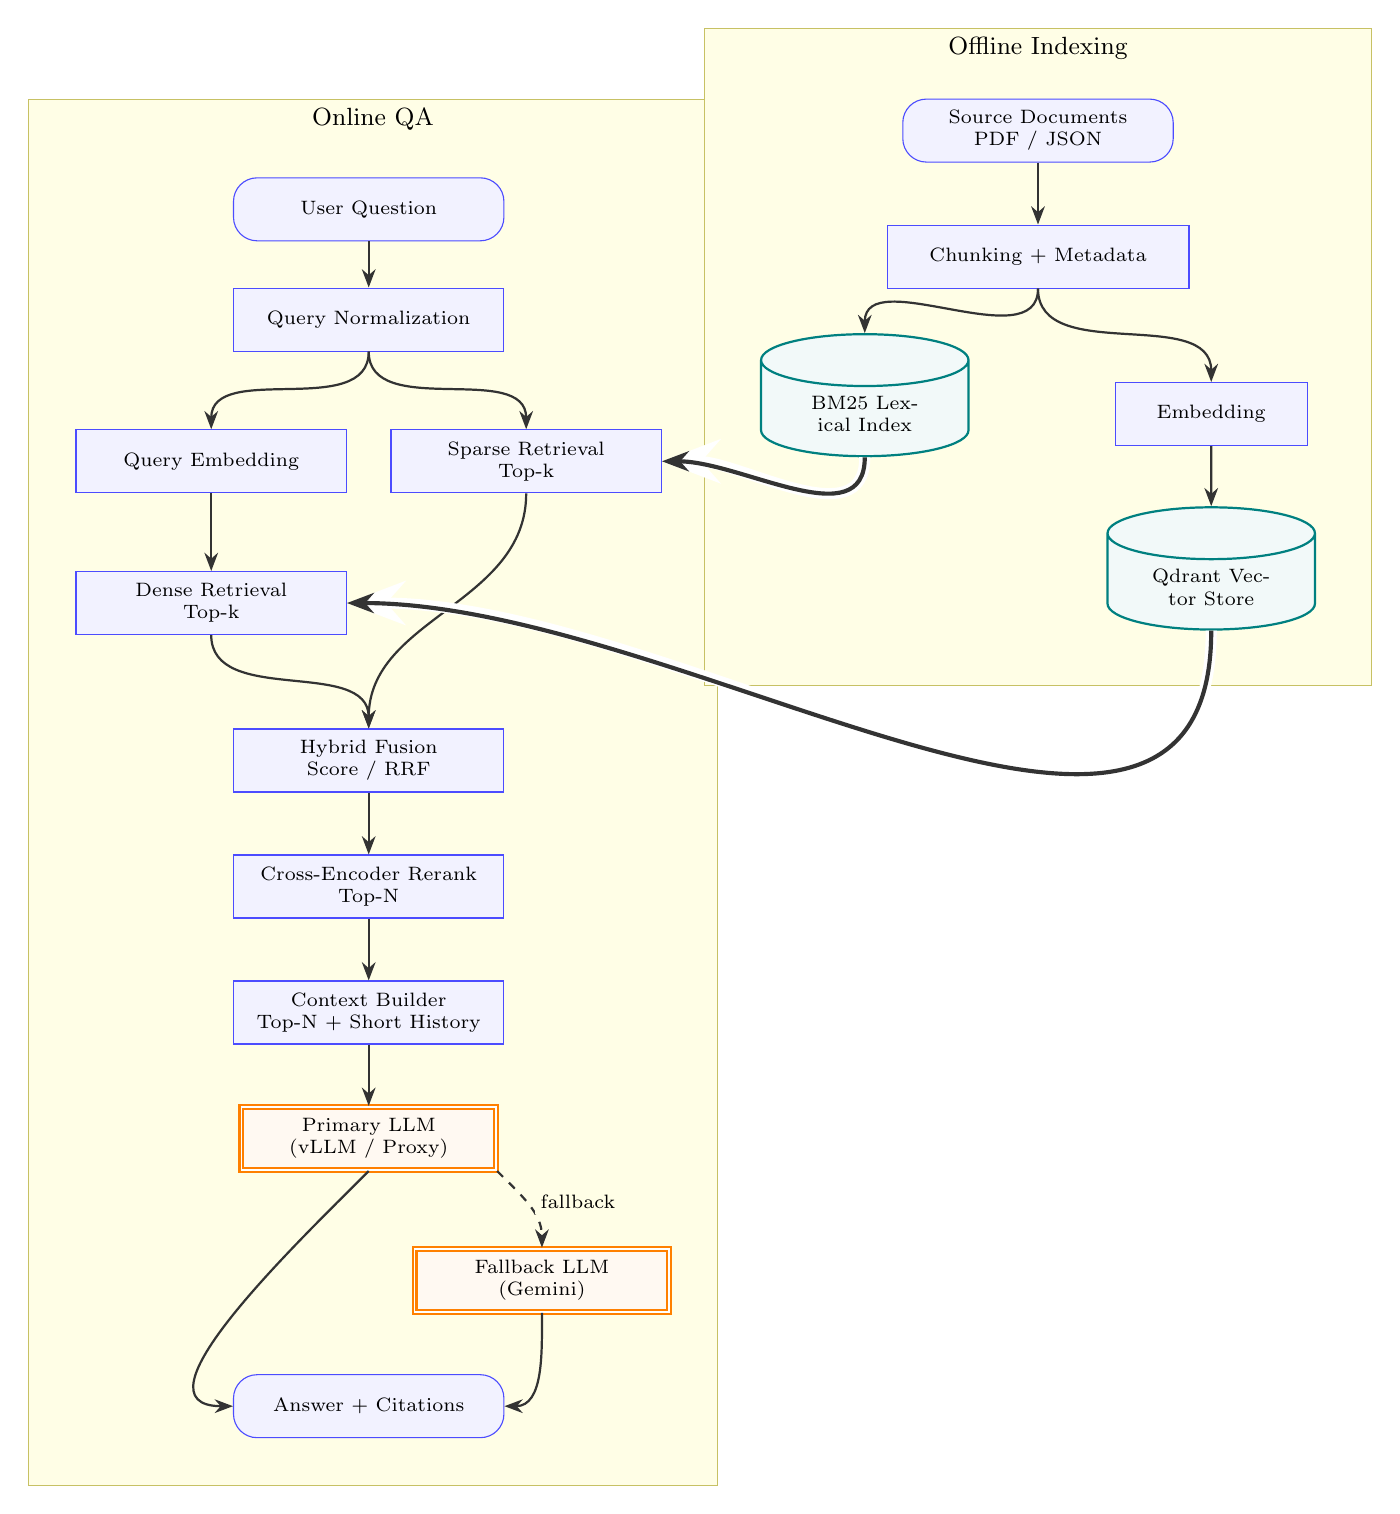
\begin{tikzpicture}[
    every node/.style={font=\scriptsize},
    base/.style={align=center, minimum height=0.8cm},
    input/.style={base, rectangle, rounded corners=3mm, draw=blue!70, fill=blue!5, text width=3.2cm},
    process/.style={base, rectangle, draw=blue!70, fill=blue!5, text width=3.2cm},
    db/.style={base, cylinder, draw=teal, thick, shape border rotate=90, aspect=0.25, fill=teal!5, text width=2.4cm},
    llm/.style={base, rectangle, draw=orange, thick, double, fill=orange!5, text width=3.0cm},
    arrow/.style={->, >=Stealth, thick, draw=black!80},
    thickarrow/.style={->, >=Stealth, line width=1.5pt, draw=black!80},
    dashedarrow/.style={->, >=Stealth, thick, dashed, draw=black!80}
]

\node[input] (UQ) at (0, 0) {User Question};
\node[process] (QN) at (0, -1.4) {Query Normalization};
\node[process] (QE) at (-2.0, -3.2) {Query Embedding};
\node[process] (SR) at (2.0, -3.2) {Sparse Retrieval\\Top-k};
\node[process] (DR) at (-2.0, -5.0) {Dense Retrieval\\Top-k};

\node[process] (HF) at (0, -7.0) {Hybrid Fusion\\Score / RRF};
\node[process] (CR) at (0, -8.6) {Cross-Encoder Rerank\\Top-N};
\node[process] (CB) at (0, -10.2) {Context Builder\\Top-N + Short History};

\node[llm] (PLLM) at (0, -11.8) {Primary LLM\\(vLLM / Proxy)};
\node[llm] (FLLM) at (2.2, -13.6) {Fallback LLM\\(Gemini)};
\node[input] (ANS) at (0, -15.2) {Answer + Citations};

\node[input] (SD) at (8.5, 1.0) {Source Documents\\PDF / JSON};
\node[process, text width=3.6cm] (CM) at (8.5, -0.6) {Chunking + Metadata};
\node[db] (BM) at (6.3, -2.6) {BM25 Lexical Index};
\node[process, text width=2.2cm] (EM) at (10.7, -2.6) {Embedding};
\node[db] (QD) at (10.7, -4.8) {Qdrant Vector Store};

\begin{scope}[on background layer]
    \coordinate (TopOnline) at (0, 0.8);
    \coordinate (TopOffline) at (8.5, 1.6);
    \node[draw=olive!50, fill=yellow!10, inner xsep=0.6cm, inner ysep=0.6cm,
          fit=(TopOnline) (UQ) (ANS) (QE) (SR) (FLLM) (DR)] (BoxOnline) {};
    \node[anchor=north, font=\small] at (BoxOnline.north) {Online QA};
    \node[draw=olive!50, fill=yellow!10, inner xsep=0.7cm, inner ysep=0.7cm,
          fit=(TopOffline) (SD) (CM) (BM) (EM) (QD)] (BoxOffline) {};
    \node[anchor=north, font=\small] at (BoxOffline.north) {Offline Indexing};
\end{scope}

\draw[arrow] (UQ) -- (QN);
\draw[arrow] (QN) to[out=270, in=90] (QE);
\draw[arrow] (QN) to[out=270, in=90] (SR);
\draw[arrow] (QE) -- (DR);
\draw[arrow] (DR) to[out=270, in=90] (HF);
\draw[arrow] (SR) to[out=270, in=90] (HF);
\draw[arrow] (HF) -- (CR);
\draw[arrow] (CR) -- (CB);
\draw[arrow] (CB) -- (PLLM);
\draw[arrow] (PLLM.south) to[out=225, in=180] (ANS.west);
\draw[dashedarrow] (PLLM.south east) to[out=315, in=90]
      node[pos=0.45, right=1mm, fill=yellow!10, inner sep=2pt] {fallback} (FLLM.north);
\draw[arrow] (FLLM.south) to[out=270, in=0] (ANS.east);
\draw[arrow] (SD) -- (CM);
\draw[arrow] (CM) to[out=270, in=90] (BM);
\draw[arrow] (CM) to[out=270, in=90] (EM);
\draw[arrow] (EM) -- (QD);
\draw[thickarrow, preaction={draw, white, line width=4pt}]
    (BM.south) to[out=270, in=0] (SR.east);
\draw[thickarrow, preaction={draw, white, line width=4pt}]
    (QD.south) to[out=270, in=0] (DR.east);

\end{tikzpicture}%
}
\caption{End-to-end hybrid RAG pipeline architecture.}
\label{fig:rag_pipeline}
\end{figure}

\subsection{Data Preparation and Educational AI}

The effectiveness of retrieval-based systems is strongly influenced by the quality of the indexed knowledge base. Naive fixed-window chunking often disrupts semantic structure in technical documents containing code, formulas, or complex layouts~\cite{gao2023survey}. Recent studies on semantic segmentation and chunking show that preserving discourse-level coherence can improve embedding quality and downstream retrieval performance~\cite{duarte2024lumberchunker,qu2025semantic}. 

In educational settings, AI chatbots have increasingly been explored to support scalable learner interaction in online learning environments~\cite{winkler2020chatbots}. Retrieval-augmented approaches are particularly attractive because they constrain generation to course-specific materials and reduce hallucination compared to standalone LLMs. However, most existing educational chatbot systems rely primarily on single-stage retrieval pipelines, while the combined effects of hybrid retrieval and reranking across multiple subjects and multilingual educational content remain insufficiently studied. This gap motivates the controlled ablation analysis presented in this work.


%% ─────────────────────────────────────────────
\section{Methodology}
\label{ppmethod}
%% ─────────────────────────────────────────────

The pipeline is structured so that each stage corrects the failure mode that the preceding stage cannot address. Fig.~\ref{fig:rag_pipeline} illustrates the three-stage flow from document ingestion through retrieval to generation.

\subsection{Structured Data Ingestion}
\label{sec:ingestion}

MOOC materials are inherently multimodal; retrieval quality is bounded by ingestion fidelity, so this stage prioritises preserving semantic structure.

\begin{figure}[!t]
\centering
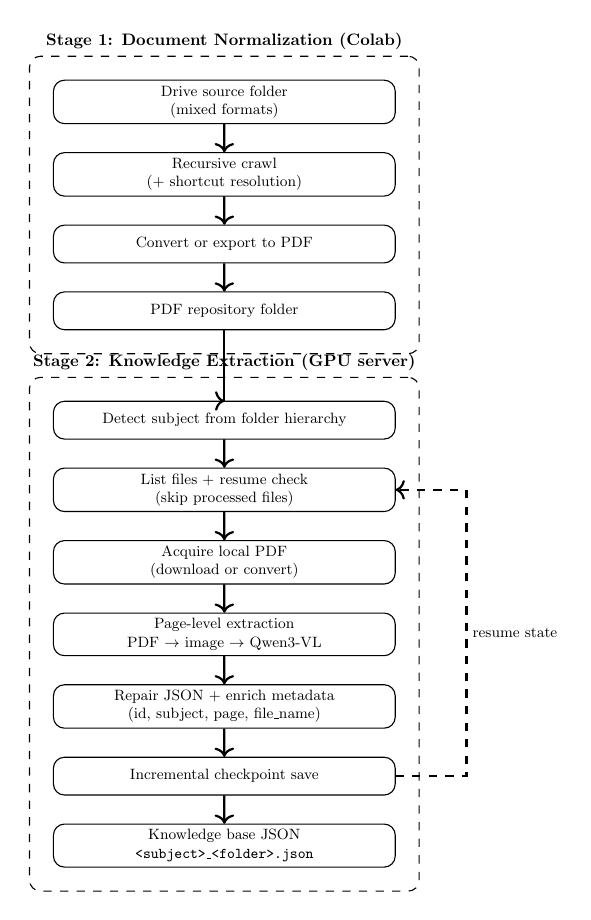
\begin{tikzpicture}[
    scale=0.6,
    transform shape,
    node distance=0.6cm,
    every node/.style={font=\small},
    block/.style={
        rectangle, draw, rounded corners,
        align=center,
        minimum height=0.8cm,
        text width=7cm
    },
    arrow/.style={->, thick},
    dashedarrow/.style={->, thick, dashed}
]

% --- Stage 1 ---
\node[block] (A) {Drive source folder\\(mixed formats)};
\node[block, below=of A] (B) {Recursive crawl\\(+ shortcut resolution)};
\node[block, below=of B] (C) {Convert or export to PDF};
\node[block, below=of C] (D) {PDF repository folder};

% Stage 1 box
\node[draw, dashed, rounded corners, fit=(A)(B)(C)(D), inner sep=0.3cm,
      label={[font=\bfseries]above:Stage 1: Document Normalization (Colab)}] (Stage1) {};

% --- Stage 2 ---
\node[block, below=1.5cm of D] (E) {Detect subject from folder hierarchy};
\node[block, below=of E] (F) {List files + resume check\\(skip processed files)};
\node[block, below=of F] (G) {Acquire local PDF\\(download or convert)};
\node[block, below=of G] (H) {Page-level extraction\\PDF $\rightarrow$ image $\rightarrow$ Qwen3-VL};
\node[block, below=of H] (I) {Repair JSON + enrich metadata\\(id, subject, page, file\_name)};
\node[block, below=of I] (J) {Incremental checkpoint save};
\node[block, below=of J] (K) {Knowledge base JSON\\\texttt{<subject>\_<folder>.json}};

% Stage 2 box
\node[draw, dashed, rounded corners, fit=(E)(F)(G)(H)(I)(J)(K), inner sep=0.3cm,
      label={[font=\bfseries]above:Stage 2: Knowledge Extraction (GPU server)}] (Stage2) {};

% --- Arrows ---
\draw[arrow] (A) -- (B);
\draw[arrow] (B) -- (C);
\draw[arrow] (C) -- (D);
\draw[arrow] (D) -- (Stage1.south |- D.south) -- (Stage2.north |- E.north) -- (E);
\draw[arrow] (E) -- (F);
\draw[arrow] (F) -- (G);
\draw[arrow] (G) -- (H);
\draw[arrow] (H) -- (I);
\draw[arrow] (I) -- (J);
\draw[arrow] (J) -- (K);

% Resume loop (vòng qua bên phải để không cắt ngang text)
\draw[dashedarrow] (J.east) -- ++(1.5,0) |- node[pos=0.25, right]{resume state} (F.east);

\end{tikzpicture}
\caption{Two-stage pipeline for document normalization and knowledge extraction.}
\label{fig:pipeline}
\end{figure}
\FloatBarrier 

\noindent\textbf{Document ingestion.} Slides and PDFs are processed by a Vision-Language Model pipeline based on Qwen3-VL-8B (bfloat16, Scaled Dot-Product Attention). Each PDF page is rasterised at 200~DPI by PyMuPDF and passed to the VLM with a structured extraction prompt that renders mathematical expressions as LaTeX, formats tables as Markdown, and preserves code indentation verbatim. A JSON repair heuristic restores syntactic validity when output is truncated at the 6,144-token generation limit. This approach avoids the multi-column layout corruption, formula truncation, and code indentation loss that affect standard OCR extractors.

\noindent\textbf{Semantic TextNode construction.} Rather than fixed-size character chunking, the pipeline produces semantically complete TextNode units. A minimum threshold of 20 words per node filters low-information artifacts (blank pages, title-only slides, administrative text), preserving semantic density in the vector database. Hash-based deduplication using a set structure removes identical strings within the same document iteration; each surviving node is then assigned a globally unique UUID~v4, preventing data collisions during asynchronous database updates.

\noindent\textbf{Embedding.} All TextNodes are encoded with BAAI/bge-m3, a multilingual model supporting Vietnamese, English, and code within a shared embedding space, loaded once at server startup to avoid repeated initialisation overhead.

\subsection{Parallel Hybrid Retrieval}
\label{sec:retrieval}

Student queries span two fundamentally different information needs: conceptual questions that benefit from semantic paraphrase matching, and precise technical lookups requiring exact keyword or identifier matching. No single retrieval mode handles both effectively, motivating concurrent dense and sparse retrieval followed by score fusion.

\noindent\textbf{Dense retrieval.} The query is encoded with BAAI/bge-m3 and a cosine similarity search is performed in Qdrant, returning the top~20 candidates with a minimum similarity threshold of~0.3. A Qdrant FieldCondition restricts retrieval to the selected course subject, preventing cross-domain hallucination.

\noindent\textbf{Sparse retrieval.} An in-memory BM25Okapi index is built at server startup. A metadata boosting algorithm duplicates technical keywords from node metadata three times (\texttt{BM25\_KEYWORD\_BOOST}~=~3) and topic classification tokens twice (\texttt{BM25\_TOPIC\_BOOST}~=~2) before indexing, ensuring domain-specific identifiers receive elevated term-frequency scores that dense retrieval generalises over. The top~20 BM25 candidates are retrieved independently.

\noindent\textbf{Score fusion.} Because cosine similarity scores are bounded in $[-1,1]$ while BM25 scores are unbounded, both distributions are min-max normalised before fusion:
\begin{equation}
s_{\text{hybrid}}(d) = \alpha \cdot s_{\text{dense}}(d) + \beta \cdot s_{\text{BM25}}(d), \quad \alpha + \beta = 1
\end{equation}
with $\alpha = 0.7$ and $\beta = 0.3$, determined empirically, prioritising semantic coverage while preserving keyword sensitivity. Reciprocal Rank Fusion (RRF)~\cite{cormack2009rrf} is supported as an alternative fusion mode. The fused candidate pool contains up to~40 nodes.

\subsection{Cross-Encoder Reranking}
\label{sec:reranking}

Hybrid retrieval maximises the probability that the relevant passage appears in the candidate pool, but the fused score may not reliably rank it first: bi-encoders approximate relevance without exploiting token-level query--document interactions.

BAAI/bge-reranker-v2-m3 processes each (query, candidate) pair jointly through shared self-attention, producing precise relevance scores. A metadata boost applies $+0.05$ for each exact keyword match and $+0.10$ for a matching topic token. The top~5 reranked nodes form the final generation context.

\noindent\textbf{Inference efficiency.} To reduce CPU latency, the system selects among three inference backends in priority order: OpenVINO, ONNX Runtime, and PyTorch. This adaptive chain achieves up to a 30.5\% latency reduction over the PyTorch baseline (Section~\ref{sec:backend}).

\subsection{Generation}

The top-5 reranked passages and the three most recent conversational turns are injected into the system prompt for Qwen3-8B-AWQ, which applies 4-bit Activation-aware Weight Quantization (AWQ), reducing VRAM requirements below 6~GB. The model is served by vLLM with PagedAttention and Continuous Batching for concurrent user sessions. A language-detection step directs the model to respond in the same language as the query (Vietnamese or English).

%% ─────────────────────────────────────────────
\FloatBarrier
\section{Experiments}
\label{expeval}
%% ─────────────────────────────────────────────

\subsection{Dataset}

All course materials were collected from the VNU-HCM MOOC platform~\footnote{https://mooc.vnuhcm.edu.vn}. The evaluation spans four subjects across different domains, document structures, and language settings. Three courses are in Vietnamese, while Object-Oriented Programming is primarily English-based and contains more code-oriented content. For each subject, 100 evaluation queries were constructed from course materials and manually verified to reflect realistic student information needs. Query generation was initially assisted by LLMs to improve topical coverage, but all queries, relevance judgments, and reference answers were fully reviewed and corrected manually. Queries were stratified by type and difficulty. Multiple chunks could be labeled as relevant when they provided semantically equivalent explanations or alternative formulations of the same concept, preventing penalization of valid retrieval variations. Table~\ref{tab:dataset} summarises the evaluation dataset.

\begin{table}[ht]
\caption{Evaluation dataset with 100 annotated queries per subject.}
\label{tab:dataset}
\centering
\begin{tabular}{|p{3cm}|l|p{4.5cm}|c|c|c|}
\hline
\textbf{Subject} & \textbf{Language} & \textbf{Primary Query Types} & \textbf{Easy} & \textbf{Med.} & \textbf{Hard} \\
\hline

Marxist-Leninist Philosophy
& Vietnamese
& definition, reasoning, comparison, application
& 33\%
& 54\%
& 13\% \\
\hline

Introduction to Artificial Intelligence
& Vietnamese
& conceptual, algorithmic, factual, example-based
& 27\%
& 51\%
& 22\% \\
\hline

Object-Oriented Programming
& English
& conceptual, factual, application-oriented
& 45\%
& 40\%
& 15\% \\
\hline

Physics 2
& Vietnamese
& factual, mathematical reasoning
& 35\%
& 57\%
& 8\% \\
\hline

\end{tabular}
\end{table}

\FloatBarrier

\subsection{Evaluation Metrics}

Retrieval quality is measured using six rank-based metrics over the top-8 results. MRR captures the average reciprocal rank of the first relevant chunk. Hit@$k$ ($k \in {1,3,8}$) measures whether at least one relevant chunk appears within the top-$k$ results, while Recall@8 measures the coverage of all annotated relevant chunks in the top-8 list. nDCG@8 further accounts for the position of relevant chunks, rewarding higher-ranked relevance. Generation quality is evaluated using the RAGAS framework. Faithfulness measures whether generated outputs are supported by retrieved evidence, while Answer Correctness evaluates semantic and factual alignment with reference answers.

Qwen3-8B-AWQ is used both as generator and evaluation judge. Since the same model family is used for both roles, RAGAS scores should be interpreted as relative indicators rather than absolute human judgments. Generation uses the top-3 reranked chunks as context, while retrieval metrics are computed over the top-8 candidates to decouple retrieval quality from generation effects.

\subsection{Ablation Configurations}

Four configurations are evaluated in a strict incremental setting. The embedding model, BM25 index, and reranker weights remain fixed across all experiments; only the retrieval pipeline differs.

\begin{itemize}

\item \textbf{Config 1 -- Dense Retrieval}: bi-encoder retrieval only without reranking, serving as the conventional dense RAG baseline.

\item \textbf{Config 2 -- Hybrid Retrieval}: combines dense retrieval and BM25 lexical retrieval using a weighted score fusion with min-max normalization, without reranking.

\item \textbf{Config 3 -- Dense Retrieval + Reranking}: applies cross-encoder reranking to the dense-retrieval candidate pool, isolating reranking benefits without recall expansion from BM25.

\item \textbf{Config 4 -- Full Pipeline}: combines hybrid retrieval and cross-encoder reranking in the final production configuration.

\end{itemize}

All configurations use BAAI/bge-m3 for dense retrieval, BAAI/bge-reranker-v2-m3 for reranking, and Qwen3-8B-AWQ for generation. The models were selected for their multilingual capabilities and strong support for Vietnamese and English educational content. Generation metrics are excluded from the component-wise ablation analysis to isolate retrieval behaviour.

\subsection{Structured Data Ingestion}

Before indexing, all MOOC materials are transformed into structured TextNodes through a preprocessing pipeline designed for heterogeneous educational content. Presentation slides and PDF materials are processed using a Vision-Language Model (VLM)-based extraction pipeline that preserves semantic structure, mathematical notation, and layout information more effectively than conventional OCR-based methods.

Each TextNode stores cleaned content together with metadata such as course, source file, and section information. Deterministic UUID-based identifiers enable incremental indexing and efficient knowledge-base updates without full reprocessing.
%% ─────────────────────────────────────────────
\FloatBarrier
\section{Results and Discussion}
\label{resdis}
%% ─────────────────────────────────────────────

\subsection{Full Pipeline Performance}

Table~\ref{tab:full_pipeline} presents the complete metric matrix for the full production pipeline at top-$k = 8$. Three retrieval performance tiers are evident.

\begin{table}[ht]
\caption{Full pipeline results across four subjects.}
\label{tab:full_pipeline}
\centering
\begin{tabular}{|l|c|c|c|c|}
\hline
Metric & Philosophy & AI Intro & OOP & Physics 2 \\
\hline
Recall@8        & 0.9042 & 0.9517 & 0.8150 & 0.9400 \\
MRR             & 0.9076 & 0.8690 & 0.5885 & 0.7375 \\
Hit@1           & 0.85   & 0.78   & 0.42   & 0.70   \\
Hit@3           & 0.96   & 0.96   & 0.73   & 0.88   \\
Hit@8           & 0.99   & 0.99   & 0.84   & 0.94   \\
nDCG@8          & 0.8647 & 0.8588 & 0.6392 & 0.7861 \\
Faithfulness    & 0.9027 & 0.8706 & 0.9466 & 0.9275 \\
Ans.~Correctness & 0.7841 & 0.7588 & 0.7699 & 0.7709 \\
\hline
\end{tabular}
\end{table}

\textbf{Tier 1 -- Philosophy and AI Intro} both achieve Hit@8 = 0.99 and Recall@8 above 0.90, indicating consistently strong retrieval coverage. These Vietnamese-language subjects contain semantically coherent passages and domain-specific terminology that benefit from the combined dense and lexical retrieval strategy. Philosophy achieves the highest MRR (0.9076), suggesting that the reranker can reliably identify the most relevant passage despite substantial lexical overlap between candidate chunks.

\textbf{Tier 2 -- Physics 2} (Hit@8 = 0.94, Recall@8 = 0.94) shows substantially lower MRR (0.7375) and Hit@1 (0.70). The gap between Hit@1 and Hit@3 suggests increased ranking ambiguity in Physics~2. Many concepts are represented across multiple semantically similar passages, including differential forms, integral derivations, and worked examples of the same physical law. This makes top-rank discrimination more difficult despite consistently retrieving relevant context within the top-3 results.

\textbf{Tier 3 -- OOP} achieves the lowest retrieval performance among the four subjects (Hit@8 = 0.84, MRR = 0.5885). Although OOP and Physics~2 are both technically structured courses, the lower OOP performance may stem from multiple interacting factors, including English-language content, code-heavy materials, annotation difficulty, or reduced embedding robustness for technical terminology. Nevertheless, OOP achieves the highest faithfulness score (0.9466), indicating that once relevant context is retrieved, the generator produces highly grounded responses. This suggests that retrieval quality, rather than generation quality, remains the primary bottleneck for this subject.

Answer Correctness remains relatively stable across subjects (0.7588--0.7841) despite larger variation in retrieval metrics. This suggests that once sufficiently relevant context appears within the top-3 retrieved passages, generation quality becomes less sensitive to precise ranking order.
\FloatBarrier
\subsection{Ablation Study}

\noindent\textbf{Pattern 1: Hybrid retrieval improves recall proportionally to keyword density.} BM25 augmentation consistently raises Recall@k and Hit@k, with gains proportional to the density of exact technical vocabulary. The improvement is largest in Physics~2 (+5.0~pp Recall@k, 0.895$\to$0.945), where the BM25 index matches Vietnamese physics terminology and formula identifiers verbatim. In AI, Hit@k rises from 0.96 to 0.99 as algorithm names and acronyms benefit from exact lexical matching. For OOP, the gain is modest (Hit@k: 0.80$\to$0.81), consistent with reduced BM25 metadata-boost effectiveness for English content. For Philosophy, where dense retrieval already achieves near-ceiling recall (0.889), the hybrid gain is correspondingly smaller (0.901), demonstrating a diminishing-returns relationship. Table~\ref{tab:ablation_all} presents ablation results across all four subjects. The ablation results reveal three consistent patterns across subjects.

\noindent\textbf{Pattern 2: Reranking improves top-rank precision most in technically structured subjects.} Cross-encoder reranking consistently improves MRR, Hit@1, Hit@3, and nDCG@k relative to both the dense baseline and hybrid configuration. The effect is most pronounced in AI: MRR improves by +6.45~pp (0.8025$\to$0.8670) and Hit@1 by +10~pp (0.68$\to$0.78), as the cross-encoder exploits token-level analysis of pseudocode steps, complexity notation, and technical definitions. In OOP, Hit@3 improves from 0.66 to 0.72, while MRR remains nearly unchanged, confirming that reranking refines the ranking of retrieved candidates but cannot compensate for the retrieval gap caused by cross-lingual embedding weakness.

\begin{table}[!t]
\caption{Ablation study results across all four subjects.}
\label{tab:ablation_all}
\centering
\begin{tabular}{l@{\hspace{8pt}}c@{\hspace{8pt}}c@{\hspace{8pt}}c@{\hspace{8pt}}c}
\toprule
\textbf{Metric} & \textbf{Dense} & \textbf{Hybrid} & \textbf{Dense +} & \textbf{Hybrid +} \\
 & \textbf{Retrieval} & \textbf{Retrieval} & \textbf{Reranking} & \textbf{Reranking} \\
\midrule
\multicolumn{5}{c}{\textbf{Object-Oriented Programming}} \\
\midrule
MRR        & 0.5818 & 0.5785 & 0.5792 & 0.5885 \\
Recall@k   & 0.7500 & 0.7800 & 0.7750 & 0.8150 \\
Hit@1      & 0.46   & 0.43   & 0.42   & 0.42   \\
Hit@3      & 0.66   & 0.71   & 0.72   & 0.73   \\
Hit@k      & 0.80   & 0.81   & 0.81   & 0.84   \\
NDCG@k     & 0.6132 & 0.6183 & 0.6251 & 0.6392 \\
\midrule
\multicolumn{5}{c}{\textbf{Introduction to Artificial Intelligence}} \\
\midrule
MRR        & 0.8025 & 0.8174 & 0.8670 & 0.8690 \\
Recall@k   & 0.9083 & 0.9500 & 0.9383 & 0.9517 \\
Hit@1      & 0.68   & 0.70   & 0.78   & 0.78   \\
Hit@3      & 0.92   & 0.92   & 0.96   & 0.96   \\
Hit@k      & 0.96   & 0.99   & 0.98   & 0.99   \\
NDCG@k     & 0.7965 & 0.8238 & 0.8498 & 0.8588 \\
\midrule
\multicolumn{5}{c}{\textbf{Physics 2}} \\
\midrule
MRR        & 0.7019 & 0.7416 & 0.7348 & 0.7375 \\
Recall@k   & 0.8950 & 0.9450 & 0.9250 & 0.9400 \\
Hit@1      & 0.58   & 0.62   & 0.60   & 0.60   \\
Hit@3      & 0.83   & 0.85   & 0.88   & 0.88   \\
Hit@k      & 0.90   & 0.95   & 0.93   & 0.94   \\
NDCG@k     & 0.7425 & 0.7859 & 0.7795 & 0.7861 \\
\midrule
\multicolumn{5}{c}{\textbf{Marxist--Leninist Philosophy}} \\
\midrule
MRR        & 0.9120 & 0.9053 & 0.9082 & 0.9076 \\
Recall@k   & 0.8892 & 0.9008 & 0.8992 & 0.9042 \\
Hit@1      & 0.86   & 0.85   & 0.85   & 0.85   \\
Hit@3      & 0.96   & 0.95   & 0.96   & 0.96   \\
Hit@k      & 0.99   & 0.98   & 0.99   & 0.99   \\
NDCG@k     & 0.8627 & 0.8620 & 0.8629 & 0.8649 \\
\bottomrule
\end{tabular}
\end{table}

\FloatBarrier

\noindent\textbf{Pattern 3: The full pipeline combines orthogonal benefits.} The full pipeline achieves the best or jointly best scores on the majority of metrics for all four subjects. The gains are additive: BM25 expands the candidate pool and reduces coverage failures (low Recall@k, Hit@k), while the cross-encoder reorders the expanded pool to reduce ranking errors (low MRR, Hit@1). These failure modes are structurally orthogonal---adding BM25 without reranking slightly reduces MRR in OOP (0.5818$\to$0.5785) because the fused score occasionally promotes lexically similar but contextually weaker chunks; the cross-encoder corrects this. Conversely, reranking alone cannot compensate for candidates absent from the narrow dense-only pool. For AI, the full pipeline is strictly dominant across all six metrics simultaneously (MRR = 0.8690, Recall@k = 0.9517, nDCG@k = 0.8588), providing the clearest evidence of complementarity.

\noindent\textbf{Domain sensitivity.} Technical subjects (AI and Physics~2) exhibit the largest absolute gains from both mechanisms, as terminology-rich content creates sharp vocabulary boundaries for BM25 and sharp relevance distinctions for the cross-encoder. Philosophy shows near-identical performance across all four configurations (MRR range: 0.9053--0.9120; nDCG@k range: 0.8620--0.8649), indicating that dense retrieval already saturates available retrieval signal for philosophically abstract Vietnamese text. These results suggest that hybrid retrieval and reranking are most beneficial in technically structured subjects containing dense terminology, formulas, or acronym-heavy content.
\FloatBarrier
\subsection{Reranker Backend Benchmark}
\label{sec:backend}

Table~\ref{tab:backend} presents benchmark results across three inference backends on an Intel Xeon server (48 query--passage pairs per run, five repeated runs).

\begin{table}[ht]
\caption{Reranker backend benchmark results.}
\label{tab:backend}
\centering
\begin{tabular}{|l|c|c|c|}
\hline
Metric & PyTorch (baseline) & ONNX Runtime & OpenVINO \\
\hline
Avg Latency (ms)    & 7,507.54 & 5,635.22 & 5,214.74 \\
P50 (ms)            & 7,488.74 & 5,635.59 & 5,205.31 \\
P95 (ms)            & 7,568.91 & 5,703.47 & 5,378.67 \\
Throughput (pairs/s)& 6.39     & 8.52     & 9.20     \\
\hline
\end{tabular}
\end{table}


ONNX Runtime reduces average latency by 24.9\% over PyTorch (7,508$\to$5,635~ms), raising throughput from 6.39 to 8.52 pairs/s. OpenVINO achieves a further 7.4\% improvement (5,215~ms, 9.20~pairs/s), for a 30.5\% total reduction. The P50-to-P95 spread stays below 200~ms for all backends. At the default pool size of 20 nodes, OpenVINO completes reranking in approximately 2.2~s, an acceptable contribution to end-to-end latency given the precision gains quantified in the ablation study.
\FloatBarrier
\subsection{Discussion}

Three observations emerge from the results. First, hybrid retrieval and cross-encoder reranking provide complementary benefits by addressing different retrieval failure modes. Hybrid retrieval improves coverage through lexical matching, while reranking improves the ordering of semantically similar candidates. Second, component effectiveness is domain-dependent. In subjects where dense retrieval already achieves high recall, BM25 contributes only marginal gains. In technically structured subjects containing formulas, acronyms, or specialised terminology, hybrid retrieval improves Recall@8 by more than 5 percentage points. This suggests retrieval configurations should be adapted to course characteristics rather than uniformly applied across domains. Third, retrieval quality remains constrained by ingestion quality. The VLM-based extraction pipeline produces semantically coherent TextNodes with structural metadata that support both embedding and lexical retrieval. Errors introduced during ingestion propagate throughout later retrieval stages and are difficult to correct downstream.

This study still possesses several limitations. Lower OOP performance may reflect reduced robustness for English technical content, although code-heavy materials and annotation difficulty may also contribute. In Physics~2, semantically equivalent passages describing the same physical law make top-rank discrimination difficult despite high retrieval coverage. In addition, ASR-based ingestion still introduces transcription noise that current filtering methods only partially mitigate.
%% ─────────────────────────────────────────────
\section{Conclusion}
\label{conclusion}
%% ─────────────────────────────────────────────

This paper investigated the effectiveness of multi-stage retrieval architectures for educational question answering on MOOC platforms. Through controlled ablation experiments across four subjects and 400 annotated queries, the study shows that hybrid dense--lexical retrieval and cross-encoder reranking address different retrieval failure modes and provide complementary improvements when combined within a unified RAG pipeline.

The results indicate that retrieval enhancement is strongly domain-dependent. Hybrid retrieval contributes most in terminology-rich technical subjects, while reranking is particularly effective when semantically similar passages require finer relevance discrimination. In contrast, gains become marginal in domains where dense retrieval already achieves near-saturated recall. The findings suggest that multi-stage retrieval pipelines provide a practical and scalable approach for grounding educational AI assistants in heterogeneous MOOC content. Remaining challenges include cross-lingual retrieval robustness, disambiguation among mathematically equivalent passages, and improved noise reduction for ASR-derived educational materials.

%\begin{credits}
%\subsubsection{\ackname}
%The authors thank the research staff and fellow students at the Institute of Information Technology and Programming (ITP), The International University, VNU-HCM. The authors are particularly grateful to Tran Manh Ha, Ph.D., Associate Professor, for his leadership and guidance, and to Nguyen Huu Viet Long, M.Sc., for initiating the work and providing technical and evaluation support. The authors also acknowledge Ho Long Van, Ph.D., for his contributions to this study.
%\end{credits}

\begin{thebibliography}{16}

\bibitem{lewis2020rag}
Lewis, P., et al.: Retrieval-Augmented Generation for Knowledge-Intensive NLP Tasks. In: Advances in Neural Information Processing Systems (NeurIPS) (2020). \url{https://arxiv.org/pdf/2005.11401}

\bibitem{gao2023survey}
Gao, Y., et al.: Retrieval-Augmented Generation for Large Language Models: A Survey. arXiv preprint arXiv:2312.10997 (2023). \url{https://arxiv.org/abs/2312.10997}

\bibitem{robertson2009bm25}
Robertson, S., Zaragoza, H.: The Probabilistic Relevance Framework: BM25 and Beyond. Foundations and Trends in Information Retrieval \textbf{3}(4), 333--389 (2009). \doi{10.1561/1500000019}

\bibitem{cormack2009rrf}
Cormack, G.V., Clarke, C.L.A., B\"{u}ttcher, S.: Reciprocal Rank Fusion Outperforms Condorcet and Individual Rank Learning Methods. In: Proc. SIGIR (2009). \doi{10.1145/1571941.1572114}

\bibitem{reimers2019sbert}
Reimers, N., Gurevych, I.: Sentence-BERT: Sentence Embeddings using Siamese BERT-Networks. In: Proc. EMNLP (2019). \url{https://arxiv.org/abs/1908.10084}

\bibitem{bgem3}
Chen, J., et al.: BGE-M3: Multi-Lingual, Multi-Functionality, Multi-Granularity Text Embeddings Through Self-Knowledge Distillation. arXiv preprint arXiv:2402.03216 (2024). \url{https://arxiv.org/abs/2402.03216}

\bibitem{wang2020minilm}
Wang, W., et al.: MiniLM: Deep Self-Attention Distillation for Task-Agnostic Compression of Pre-Trained Transformers. In: Advances in Neural Information Processing Systems (NeurIPS) (2020). \url{https://arxiv.org/abs/2002.10957}

\bibitem{guu2020realm}
Guu, J., et al.: REALM: Retrieval-Augmented Language Model Pre-Training. In: Proc. ICML (2020). \url{https://arxiv.org/abs/2002.08909}

\bibitem{izacard2021leveraging}
Izacard, G., Grave, E.: Leveraging Passage Retrieval with Generative Models for Open Domain Question Answering. In: Proc. ICLR (2021). \url{https://arxiv.org/abs/2007.01282}

\bibitem{ram2023incontext}
Ram, O., et al.: In-Context Retrieval-Augmented Language Models. Transactions of the ACL \textbf{11}, 1316--1331 (2023). \doi{10.1162/tacl\_a\_00577}

\bibitem{ma2021dense}
Ma, X., et al.: Dense-Sparse Hybrid Retrieval for Open-Domain Question Answering. In: Findings of ACL (2021). \url{https://arxiv.org/abs/2106.00882}

\bibitem{nogueira2019passage}
Nogueira, R., Cho, K.: Passage Re-ranking with BERT. arXiv preprint arXiv:1901.04085 (2019). \url{https://arxiv.org/abs/1901.04085}

\bibitem{duarte2024lumberchunker}
Duarte, A.V., et al.: LumberChunker: Long-Form Narrative Document Segmentation. In: Findings of EMNLP (2024). \url{https://aclanthology.org/2024.findings-emnlp.377/}

\bibitem{qu2025semantic}
Qu, R., et al.: Is Semantic Chunking Worth the Computational Cost? In: Findings of NAACL (2025). \url{https://aclanthology.org/2025.findings-naacl.114/}

\bibitem{winkler2020chatbots}
Winkler, A., S\"{o}llner, H.: Unleashing the Potential of Chatbots in Education: A State-of-the-Art Analysis. Computers \& Education: Artificial Intelligence \textbf{1} (2020). \doi{10.1016/j.caeai.2020.100002}

\end{thebibliography}

\end{document}